%%%%%%%%%%%%%%%%%%%%%%%%%%%%%%%%%%%%%%%%%
%
% 
%
%%%%%%%%%%%%%%%%%%%%%%%%%%%%%%%%%%%%%%%%%

%----------------------------------------------------------------------------------------
%	PACKAGES AND OTHER DOCUMENT CONFIGURATIONS
%----------------------------------------------------------------------------------------

\documentclass[paper=a4, fontsize=11pt]{scrartcl} % A4 paper and 11pt font size
\usepackage[]{algorithm2e} % Used for loading the algorithm package

%=-----------------------for diagram ---------
\usepackage{graphicx}

\usepackage{cite}	%for bibtex
\usepackage{hyperref}	%for crossreferencing inside text
\usepackage{url}	%for urls

\usepackage{listings} % Required for inserting code snippets
\usepackage[usenames,dvipsnames]{color} % Required for specifying custom colors and referring to colors by name
\definecolor{DarkGreen}{rgb}{0.0,0.4,0.0} % Comment color
\definecolor{highlight}{RGB}{255,251,204} % Code highlight color

\lstdefinestyle{Style1}{ % Define a style for your code snippet, multiple definitions can be made if, for example, you wish to insert multiple code snippets using different programming languages into one document
language=Java, % Detects keywords, comments, strings, functions, etc for the language specified
backgroundcolor=\color{highlight}, % Set the background color for the snippet - useful for highlighting
basicstyle=\footnotesize\ttfamily, % The default font size and style of the code
breakatwhitespace=false, % If true, only allows line breaks at white space
breaklines=true, % Automatic line breaking (prevents code from protruding outside the box)
captionpos=b, % Sets the caption position: b for bottom; t for top
commentstyle=\usefont{T1}{pcr}{m}{sl}\color{DarkGreen}, % Style of comments within the code - dark green courier font
deletekeywords={}, % If you want to delete any keywords from the current language separate them by commas
%escapeinside={\%}, % This allows you to escape to LaTeX using the character in the bracket
firstnumber=1, % Line numbers begin at line 1
frame=single, % Frame around the code box, value can be: none, leftline, topline, bottomline, lines, single, shadowbox
frameround=tttt, % Rounds the corners of the frame for the top left, top right, bottom left and bottom right positions
keywordstyle=\color{Blue}\bf, % Functions are bold and blue
morekeywords={}, % Add any functions no included by default here separated by commas
numbers=left, % Location of line numbers, can take the values of: none, left, right
numbersep=10pt, % Distance of line numbers from the code box
numberstyle=\tiny\color{Gray}, % Style used for line numbers
rulecolor=\color{black}, % Frame border color
showstringspaces=false, % Don't put marks in string spaces
showtabs=false, % Display tabs in the code as lines
stepnumber=5, % The step distance between line numbers, i.e. how often will lines be numbered
stringstyle=\color{Purple}, % Strings are purple
tabsize=2, % Number of spaces per tab in the code
}

% Create a command to cleanly insert a snippet with the style above anywhere in the document
\newcommand{\insertcode}[2]{\begin{itemize}\item[]\lstinputlisting[caption=#2,label=#1,style=Style1]{#1}\end{itemize}} % The first argument is the script location/filename and the second is a caption for the listing



\usepackage[a4paper,pdftex]{geometry}	% Use A4 paper margins
\usepackage[english]{babel}
\usepackage{xcolor} % Required for specifying custom colors
\usepackage{fix-cm} % Allows increasing the font size of specific fonts beyond LaTeX default specifications

\setlength{\oddsidemargin}{0mm} % Adjust margins to center the colored title box
\setlength{\evensidemargin}{0mm} % Margins on even pages - only necessary if adding more content to this template

\newcommand{\HRule}[1]{\hfill \rule{0.2\linewidth}{#1}} % Horizontal rule at the bottom of the page, adjust width here

\definecolor{grey}{rgb}{1,0.9,0.6} % Color of the box surrounding the title - these values can be changed to give the box a different color	


%\usepackage{hyperref} %used for embedding url
\usepackage[T1]{fontenc} % Use 8-bit encoding that has 256 glyphs
\usepackage{fourier} % Use the Adobe Utopia font for the document - comment this line to return to the LaTeX default
\usepackage[english]{babel} % English language/hyphenation
\usepackage{amsmath,amsfonts,amsthm} % Math packages

\usepackage{lipsum} % Used for inserting dummy 'Lorem ipsum' text into the template

\usepackage{sectsty} % Allows customizing section commands
\allsectionsfont{\centering \normalfont\scshape} % Make all sections centered, the default font and small caps

\usepackage{fancyhdr} % Custom headers and footers
\pagestyle{fancyplain} % Makes all pages in the document conform to the custom headers and footers
\fancyhead{} % No page header - if you want one, create it in the same way as the footers below
\fancyfoot[L]{} % Empty left footer
\fancyfoot[C]{} % Empty center footer
\fancyfoot[R]{\thepage} % Page numbering for right footer
\renewcommand{\headrulewidth}{0pt} % Remove header underlines
\renewcommand{\footrulewidth}{0pt} % Remove footer underlines
\setlength{\headheight}{13.6pt} % Customize the height of the header

\numberwithin{equation}{section} % Number equations within sections (i.e. 1.1, 1.2, 2.1, 2.2 instead of 1, 2, 3, 4)
\numberwithin{figure}{section} % Number figures within sections (i.e. 1.1, 1.2, 2.1, 2.2 instead of 1, 2, 3, 4)
\numberwithin{table}{section} % Number tables within sections (i.e. 1.1, 1.2, 2.1, 2.2 instead of 1, 2, 3, 4)

\setlength\parindent{0pt} % Removes all indentation from paragraphs - comment this line for an assignment with lots of text

%----------------------------------------------------------------------------------------
%	TITLE SECTION
%----------------------------------------------------------------------------------------

\newcommand{\horrule}[1]{\rule{\linewidth}{#1}} % Create horizontal rule command with 1 argument of height

\title{	
\normalfont \normalsize 
\textsc{Indian Institute of Technology, Kanpur, CSE} \\ [25pt] % Your university, school and/or department name(s)
\horrule{0.5pt} \\[0.4cm] % Thin top horizontal rule
\huge CS698D, Assignment 1  \\ % The assignment title
\horrule{2pt} \\[0.5cm] % Thick bottom horizontal rule
}

\author{Harshit Maheshwari} % Your name

\date{\normalsize\today} % Today's date or a custom date

\begin{document}
%\maketitle
\thispagestyle{empty} % Remove page numbering on this page

%----------------------------------------------------------------------------------------
%	TITLE SECTION
%----------------------------------------------------------------------------------------

\colorbox{grey}{
	\parbox[t]{1.0\linewidth}{
		\centering \fontsize{50pt}{80pt}\selectfont % The first argument for fontsize is the font size of the text and the second is the line spacing - you may need to play with these for your particular title
		\vspace*{0.7cm} % Space between the start of the title and the top of the grey box
		
		\hfill Java Extension:\\
		\hfill Automatic \\
		\hfill Type Inference\\
%		\hfill Clonable Interface\par
		
		\vspace*{0.7cm} % Space between the end of the title and the bottom of the grey box
	}
}

%----------------------------------------------------------------------------------------

\vfill % Space between the title box and author information

%----------------------------------------------------------------------------------------
%	AUTHOR NAME AND INFORMATION SECTION
%----------------------------------------------------------------------------------------

{\centering \large 
\hfill Abhimanyu Jaju \ \{\texttt{abhij@iitk.ac.in}\}\\
\hfill Harshit Maheshwari\ \{\texttt{harshitm@iitk.ac.in}\}\\
\hfill Vinit Kataria\ \{ \texttt{vinitk@iitk.ac.in}\}\\
\hfill Indian Institute of Technology, Kanpur \\
\hfill Computer Science and Engineering\\
%\hfill \texttt{harshitm@iitk.ac.in} \\

\HRule{1pt}} % Horizontal line, thickness changed here

%----------------------------------------------------------------------------------------

\clearpage % Whitespace to the end of the page


\section{Class-Responsibility-Collaboration Model\label{CRCModel}}
CRC model is a very useful model used by developers to interact and work closely together to understand the needs of users and design a preliminary software specification which acts as the basis for software development phase. A CRC model looks like shown in \ref{figure:CRCModel}.
\begin{figure}
\centering
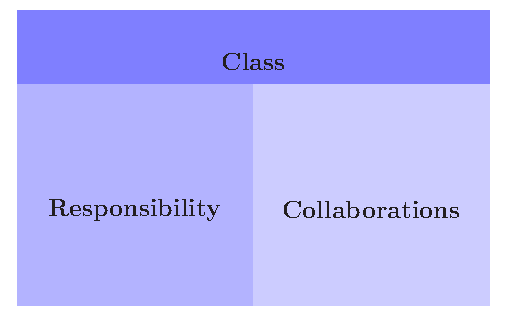
\includegraphics[width = 9cm]{crc.pdf}
\caption{CRC model\label{figure:CRCModel}}
\end{figure}
It consists of
\begin{enumerate}
	\item \textbf{Class} It is simply the class name.
	\item \textbf{Responsibility} It consists of the functions and responsibilities of the class. 
	\item \textbf{Collaborations} It consists of all the other classes that the class need in order to complete it's responsibilities. 
\end{enumerate}
For example, in \ref{figure:Animals} the class \textbf{Animals} has the \textbf{Responsibility} of eating, entertaining, excretion, sleeping and mating. In order to complete these responsibilities it has to \textbf{Collaborate} with Visitors, Admin-Animal and Cages.

\section{CRC Model for Zoo\label{ZooModel}}
While designing the CRC model for zoo we have ensured that the use of OO principles is maximized. Also, special focus has been given to code reuse and integrity of the system.
The zoo model has been designed into 4 main parts: 
\subsection{Animals\label{Animal}}
The CRC model is as shown in \ref{figure:Animals}.
\begin{figure}
\centering
\includegraphics[width = 18cm]{Animal.pdf}
\caption{CRC Model: Animals \label{figure:Animals}}
\end{figure}
As evident from the figure, there are two child classes of Animal class: Herbivores and Carnivores. Such a division is made because both the classes have same responsibilities as reflected in Animal class except the function of eating which we override in the child classes.

\subsection{Visitors\label{Visitors}}
The CRC model is as shown in \ref{figure:Visitors}.
\begin{figure}
\centering
\includegraphics[width = 18cm]{diagram2.pdf}
\caption{CRC Model: Visitors \label{figure:Visitors}}
\end{figure}
Visitors to zoo can be divided into the following types: Animal Right Activists, General Public, Health Inspectors, Media and Movie/Ad makers. Accordingly, these classes are all child classes of parent class Visitors. They all have some different functions(read responsibilities) which is reflected in \ref{figure:Visitors}.
 
\subsection{Administrative Unit\label{AdministrativeUnit}}
 The CRC model is as shown in \ref{figure:AdminUnit}.
\begin{figure}
\centering
\includegraphics[width = 18cm]{administration.pdf}
\caption{CRC Model: Administrative Unit \label{figure:AdminUnit}}
\end{figure}
The administrative unit of any zoo can be classified into the following 3 sub-types: Animal related Administration, Cleaners and Administration for people. These division have been made based on the Collaborations these classes have with other classes. The Admin-animal class is solely collaborating with Animal class, Cleaner class is collaborating with ZooStructure Class and  Admin-People class collaborates with Visitors class. 
These classes again have child classes based on their different responsibilities as shown in \ref{figure:AdminUnit}.

\subsection{Zoo Structure\label{ZooStructure}}
This part reflects the physical layout of zoo. The CRC model is as shown in \ref{figure:ZooStructure}.
\begin{figure}
\centering
\includegraphics[ width=18cm]{zooStructure.pdf}
\caption{CRC Model: Zoo Structure\label{figure:ZooStructure}}
\end{figure}
A zoo has the following physical infrastructure: cages for animals, parks, stalls and administrative buildings. The stalls can be of different types too: food stalls, sovereign shops and trivia shops. Similarly, the administrative building can be sub-divided into the following child classes: Security building, ticket booths and a main administrative block(read building). 

\section{Code Structure \label{CodeStructre}}
The entire code is available at: 
\url{https://github.com/harshitm26/Tooli-Assignments/tree/master/ZooManagementSystem/src}\\
The name of the class files is self suggestive of the functionality of the class. The following are the code files: 
\begin{enumerate}
	\item Zoo.java
	\item \textbf{ZooManagementSystem.java} - 	This is the test file which contains the main method demonstrating the use of the Zoo Management System Code. 
	\item AdministrativeUnit/AdminAnimal.java
	\item AdministrativeUnit/AdminUnit.java
	\item AdministrativeUnit/AdminPeople.java
	\item AdministrativeUnit/Cleaner.java
	\item AdministrativeUnit/Doctor.java
	\item AdministrativeUnit/Feeder.java
	\item AdministrativeUnit/SeasonalEnvironmentalist.java
	\item AdministrativeUnit/Security.java
	\item AdministrativeUnit/Service.java
	\item AdministrativeUnit/Ticket.java
	\item Animals/Animals.java
	\item Animals/Carnivores.java
	\item Animals/Elephant.java
	\item Animals/Herbivores.java
	\item Animals/Lion.java
	\item Human/Human.java
	\item Interface/Eat.java
	\item Interface/Fly.java
	\item Interface/Reproduce.java
	\item Interface/Run.java
	\item Interface/Swim.java
	\item Visitors/AnimalRightActivist.java
	\item Visitors/GeneralPublic.java
	\item Visitors/HealthInspectors.java
	\item Visitors/Media.java
	\item Visitors/MovieMakers.java
	\item Visitors/Visitors.java
	\item ZooStructure/AdminBuilding.java
	\item ZooStructure/Cages.java
	\item ZooStructure/FoodStall.java
	\item ZooStructure/Parks.java
	\item ZooStructure/SecurityBuilding.java
	\item ZooStructure/SoverignShop.java
	\item ZooStructure/Stalls.java
	\item ZooStructure/TicketBooth.java
	\item ZooStructure/Trivia.java
	\item ZooStructure/ZooStructure.java
\end{enumerate}


\end{document}